\chapter{Performance profiling at the bytecode level} % for fun and profit
\label{chap:profiling-bytecode}

%% Top-level summary
% Hook
Performance profilers are powerful tools, providing useful information about program control flow and hotspots -- facilitating performance optimisation.
% Argument
However, different circumstances demand different feature sets of these tools to ensure their users have access to the greatest amount of relevant information.
% Link
In this chapter we present ByteSight, a novel tool for performance profiling at the bytecode level, allowing us to look deeper into the performance characteristics of highly dynamic programs whose implementation cannot easily be deferred into lower level languages.

%% TODO: Need to add some stuff to the background introducing Python bytecode

%% TODO: To what degree does this duplicate related work? Will this need hoisting?
%% Research gap
% Hook
Existing profilers for Python typically operate at the function level.
% Argument
For example, Python's standard library provides the \texttt{profile} module, a Python-native tracing profiler, along with \texttt{cProfile}, a more performant C implementation of the same functionality \cite{pythonsoftwarefoundationPythonProfilers}. These instrument each call event, providing accuract profiling information for each evaluated function.
Beyond the standard library, profilers such as \texttt{pyinstrument} use statistical sampling rather than tracing to reduce overhead incurred by performance measurement \cite{rickerbyPyinstrument2025}.
Recent work such as \texttt{scalene} \cite{bergerTriangulatingPythonPerformance2023a} has focussed on the \ac{ffi} boundary between C and Python, a key bottleneck for the best practice of delegating computation to fast low-level implementations.
Whilst this delegation is particularly effective for structured workloads such as linear algebra, it is less suitable for highly dynamic workloads. % TODO: Remove whilst?
As such, profilers for pure Python are still important for these applications.
Furthermore, profiling information at a finer granularity than the function level is often needed to deeply the performance of a program.
% Link
\texttt{line\_profiler} provides this functionality to a line level \cite{robertkernPyutilsLine_profiler2025}, but this is still one level of abstraction over the increasingly complex implementation of CPython's interpreter.

% % \vspace{1em}
% \begin{listing}[H]
%     \centering
%     \begin{minted}[fontsize=\footnotesize]{text}
%       214 function calls (207 primitive calls) in 0.002 seconds

% Ordered by: cumulative time

% ncalls  tottime  percall  cumtime  percall filename:lineno(function)
%      1    0.000    0.000    0.002    0.002 {built-in method builtins.exec}
%      1    0.000    0.000    0.001    0.001 <string>:1(<module>)
%      1    0.000    0.000    0.001    0.001 __init__.py:250(compile)
%      1    0.000    0.000    0.001    0.001 __init__.py:289(_compile)
%      1    0.000    0.000    0.000    0.000 _compiler.py:759(compile)
%      1    0.000    0.000    0.000    0.000 _parser.py:937(parse)
%      1    0.000    0.000    0.000    0.000 _compiler.py:598(_code)
%      1    0.000    0.000    0.000    0.000 _parser.py:435(_parse_sub)
%     \end{minted}
%     \vspace{1em}
%     \caption{Profiling results of \texttt{cProfile.run('re.compile("foo|bar")')} are at the granularity of function calls.}
%     \label{listing:cprofile-example}
% \end{listing}

%% Bytecode intro and profiling motivation
% Hook
Recent developments to CPython's runtime motivate collecting more fine-grained profiling information.
% Argument
For example, the specialising adaptive interpreter rewrites bytecode at runtime into quickened forms, and the baseline \ac{jit} substitutes bytecode for tier two micro-operations -- both yielding performance characteristics which cannot be reasoned about with function or line level instrumentation.
In addition to this, bytecode performance profiling information helps provide a key missing data point when examining the impact of program dynamism.
However, to the author's knowledge, no profilers exist which support measurement at this granularity.
One reason for this conspicuous absence of bytecode level profilers is the difficulty of measuring their very short execution times, in the order of highest resolution system counter. This difficulty is further worsened by the bytecode dispatch and evaluation being deeply interleaved within the interpreter's execution loop.
% Link

%% Our tool and its goals
% Hook
ByteSight, our novel tool for the performance profiling of CPython bytecode, addresses this gap in the existing provision.
% Argument
ByteSight is a tracing profiler which operates on the bytecode level of the Python interpreter. It is implemented natively in Python using only the standard library, and its source code is available under the MIT license on GitHub. % s\footnote{\url{https://github.com/EdmundGoodman/bytesight}}. % TODO: This might de-anonymise me, do I need to elide it?
It does not require patches to Python's language implementation. This makes it portable, robust across language versions, and simple to install from the \ac{pypi}. % check acf here...
% Link
In this chapter, we discuss the approach and the challenges of its implementation, along with providing examples of its use.


\section{Implementation}
\label{sec:profiling-bytecode-implementation}

%% Dynamic python can be used to instrument itself
% Hook
By virtue of the flexibility and dynamism of its interpreter's implementation, CPython provides a wide variety of opportunities for instrumenting and introspecting running code.
% Argument
One example of this is the standard library function \mintinline{python}{sys.settrace}, which associates dynamic, user-defined callback functions with the dispatch of key virtual machine events. These include function calls, line execution, handling exceptions, and even individual bytecode operations (interchangeably referred to as opcodes in the documentation).
This callback function receives the event type along with the CPython frame and code objects currently being evaluated by the interpreter, facilitating precise instrumentation of the internal operation of the interpreter.
Other possibilities for collecting this information include making custom patches to the CPython implementation, or leveraging the \texttt{LLTRACE} feature of the debug build of Python.
% Link
However, the former is specific to individual language versions, and the latter has a verbose output containing no performance information. Furthermore, both requiring re-compiling the CPython implementation from source, precluding simple installation by users from \ac{pypi}.
As such, we chose to leverage \mintinline{python}{sys.settrace}, accepting the challenges associated with its measurement for benefits it provides in portability and robustness across language versions.

%% Sketch of approach
% Hook
Our tool captures bytecode level profiling information through a custom callback function which records a sequence of timestamps associated with the traced events.
% Argument
From this set of timestamps, we can calculate the execution duration of each emitted opcode. This constitutes profiling information of a higher granularity than existing Python performance profilers.
In spite of its name, we leverage the \mintinline{python}{sys.settrace} function as opposed to its sister function \mintinline{python}{sys.setprofile}. This is because \mintinline{python}{sys.settrace} has supported emitting trace events for opcodes since Python 3.7, whereas \mintinline{python}{sys.setprofile} only emits events at the function granularity.
% Link
This approach of leveraging CPython's API provides benefits of robustness across versions and easy installation, but also causes a number of challenges for accurate and precise measurement of very short events.

%% Challenges associated with approach
% Hook
These challenges come as a result of the callback function itself being a callable Python code object.
% Argument
As such, the infrastructure to invoke and evaluate this function has a significant performance cost, in many cases taking longer than the opcode it is instrumenting.
% One step that can be taken to mitigate this is implementing the callback function using Cython \cite{}, but this presents further challenges associated with crossing the \ac{ffi} boundary. % TODO: explore this more?
% Link
To navigate these challenges, we carefully co-design our tracing function with CPython's interpreter loop and tracing infrastructure in mind to exclude this overhead from the traced opode durations.


\subsection{CPython internals}
\label{ssec:profiling-bytecode-cpython-internals}

%% Interpreter loop, specific to CPython3.10. LLTrace/profile don't give us what we want
% Hook
In order to justify the validity of our tracing function, we must first examine the language runtime implementation with which it is co-designed. In this section, we present a view of CPython 3.10 as a basis for our profiler.
% Argument
In more recent Python versions such as CPython 3.13, aspects of the tracing infrastructure have been refactored. However, since both the API provided by the standard library and the position of the tracing logic in the evaluation loop remain the same, the procedure remains applicable to these newer versions.
% In background (\autoref{}) we introduced the structure of python's interpreter
Code objects in CPython are executed by the \texttt{\_PyEval\_EvalFrameDefault} function (\autoref{listing:cpython-evaluation-overview-code}). This begins with initialisation to ready for evaluation \circledbase{pairedOneLightBlue}{a}, then enters an unbounded evaluation loop \circledbase{pairedTwoDarkBlue}{b}. This loop decodes the next bytecode instruction \circledbase{pairedThreeLightGreen}{c}, then switches on it to select the appropriate logic to execute \circledbase{pairedFourDarkGreen}{d}, and repeats until an exception is thrown or the code object terminates.
% Link
Having an understanding of the evaluation loop, we can next discuss how it is instrumented for tracing.

%% Block diagram?

\begin{figure}[H]
    \centering
    \begin{subfigure}[b]{0.65\textwidth}
        \centering
        \begin{minted}[breakanywhere,fontsize=\scriptsize,escapeinside=££]{text}
PyObject* _PyEval_EvalFrameDefault(PyThreadState *tstate, PyFrameObject *f, int throwflag) {
    // ... declarations and initialization of local variables, macros definitions, call depth handling, ...  £\circledbase{pairedOneLightBlue}{\scriptsize{a}}£
    // ... code for tracing call event

    for (;;) {  £\circledbase{pairedTwoDarkBlue}{\scriptsize{b}}£
        // NEXTOPARG() macro  £\circledbase{pairedThreeLightGreen}{\scriptsize{c}}£
        _Py_CODEUNIT word = *next_instr;
        opcode = _Py_OPCODE(word);
        oparg = _Py_OPARG(word);
        next_instr++;

        // ... code for tracing opcode events

        switch (opcode) {    £\circledbase{pairedFourDarkGreen}{\scriptsize{d}}£
            case TARGET(NOP) {
                FAST_DISPATCH();
            }
            case TARGET(LOAD_FAST) {
                // ... code for loading local variable
            }
            // ... 117 more cases for every possible opcode
        }
    }
    // ... termination
}
        \end{minted}
        \captionsetup{name=Listing}
        \caption{C implementation snippets, derived from an explanation of the bytecode evaluation by Victor Skvortsov \cite{victorskvortsovPythonScenes42020}.}
        \label{listing:cpython-evaluation-overview-code}
    \end{subfigure}
    \hfill
    \begin{subfigure}[b]{0.3\textwidth}
       \centering
       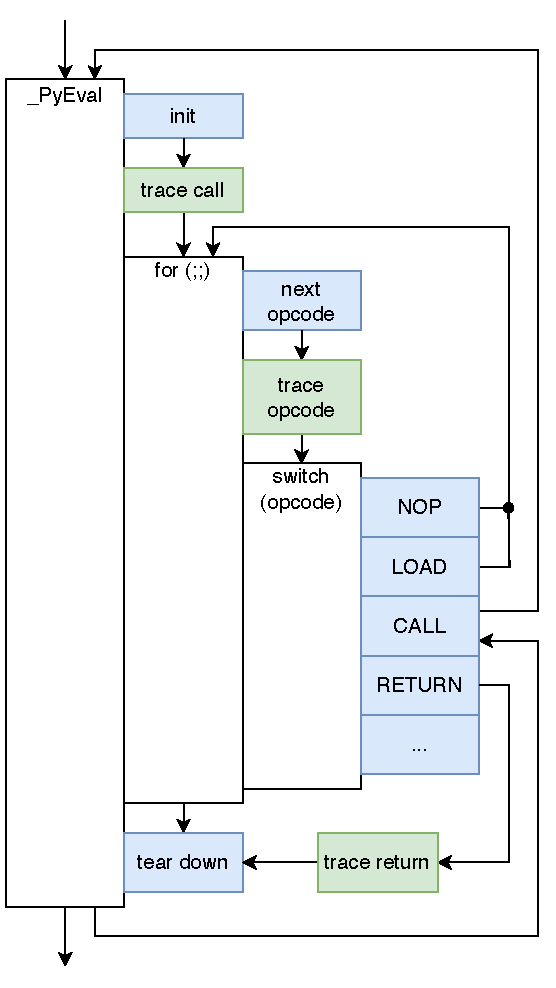
\includegraphics[width=\textwidth]{images/profiling_bytecode/python_eval.drawio.pdf}
       \vspace{1em}
       \caption{Control flow between evaluation (blue) and tracing (green).}
       \label{figure:cpython-evaluation-overview-block}
    \end{subfigure}
    \vspace{2em}
    \captionsetup{name=Listing}
    \caption{Overview of the evaluation loop of CPython 3.10, showing components relating to bytecode evaluation and tracing.}
    \label{figure:cpython-evaluation-overview}
\end{figure}


%% Registering and using a trace function
% Hook
CPython's tracing mechanism works in two phases: registering the callback function, and the invocation of this callback function from the evaluation loop.
% Argument
To register the callback function, users can invoke \mintinline{python}{sys.settrace}, a standard library function binding to the C implementation of \texttt{sys\_settrace} in \texttt{sysmodule.c:}. This in turn invokes \texttt{\_PyEval\_SetTrace} in \texttt{ceval.c}, which updates two fields on the Python \ac{gil} thread state struct: \texttt{c\_traceobj} and \texttt{c\_tracefunc}. The former is a callable Python code object for the callback function, and the latter points to a ``trampoline'' function, which invokes this code object with the current frame information.
This trampoline is then invoked when events occur in the evaluation loop, including at the start of the frame evaluation for functions, after each opcode is extracted, and on returning from the function (green blocks in \autoref{figure:cpython-evaluation-overview-block}).
% Link
As such, our approach leverages a custom callback function to sample the system timer at each event, then uses knowledge of the profiling


\subsection{Approach}
\label{ssec:profiling-bytecode-approach}

%% Our approach is...
% Hook
% Argument
% Link

%% Listing of our tracing function

% \begin{listing}[H]
%     \centering
%     \begin{minted}[breakanywhere,fontsize=\footnotesize,escapeinside=££]{text}
%     def _trace__collect_event_timestamps(
%         self, frame: types.FrameType, event: str, _arg: Any
%     ) -> Callable[..., Any] | None:
%         """Trace function to collect opcode timestamps."""
%         now_timestamp = perf_counter() £\circledbase{pairedOneLightBlue}{\footnotesize{1}}£

%         frame.f_trace_lines = False £\circledbase{pairedTwoDarkBlue}{\footnotesize{2}}£
%         frame.f_trace_opcodes = True

%         if event == "opcode":
%             self._timestamps.append( £\circledbase{pairedThreeLightGreen}{\footnotesize{3}}£
%                 (
%                     self._prev_event_timestamp,
%                     now_timestamp,
%                 )
%             )
%             self._prev_event_timestamp = perf_counter()  £\circledbase{pairedFourDarkGreen}{\footnotesize{4}}£

%         return self._trace__collect_event_timestamps
%     \end{minted}
%     \caption{.}
%     \label{listing:profiling-trace-function}
% \end{listing}

%% This gives us measurements within the CPython runtime
% Hook
This tracing function provides us with a sequence of timestamps for points in the execution stream.
% Argument
From this sequence of timestamps, we need to synthesise the durations of each opcode.
We can reason about this by flattening the block diagram of the evaluation loop (\autoref{figure:cpython-evaluation-overview-block}) and annotating it with the timestamp measurements (\autoref{}).
% Link

%% Figure showing trace events, possibly side-by-side with equations?

\begin{figure}[H]
    \centering
    \begin{subfigure}[b]{0.45\textwidth}
       \centering
       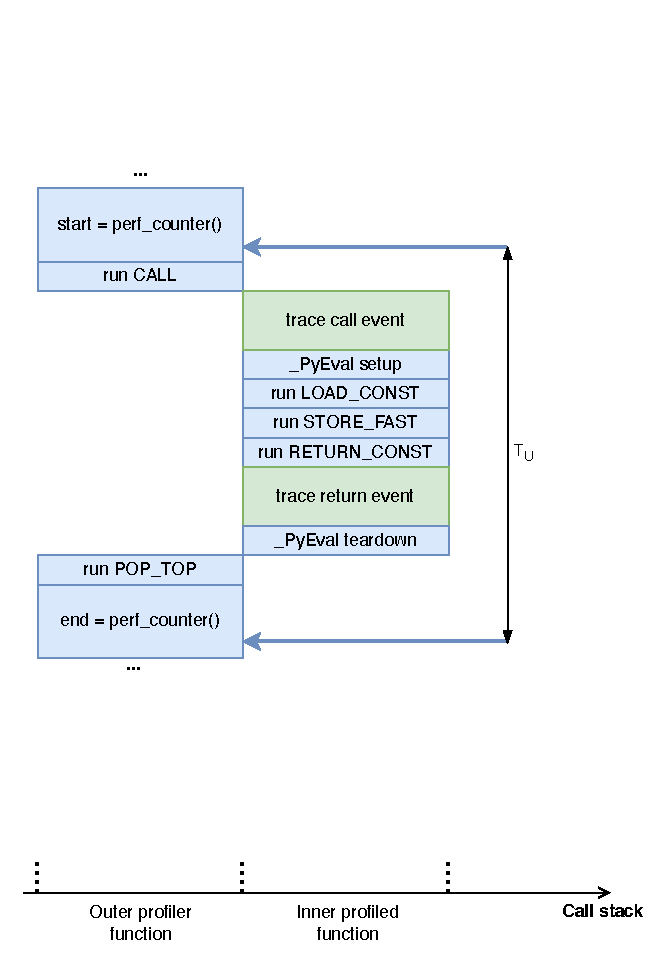
\includegraphics[width=\textwidth]{images/profiling_bytecode/untraced_run.drawio.pdf}
       \vspace{2em}
       \caption{Partially traced function.}
       \label{figure:profiler-untraced-run}
    \end{subfigure}
    \hfill
    \begin{subfigure}[b]{0.45\textwidth}
       \centering
       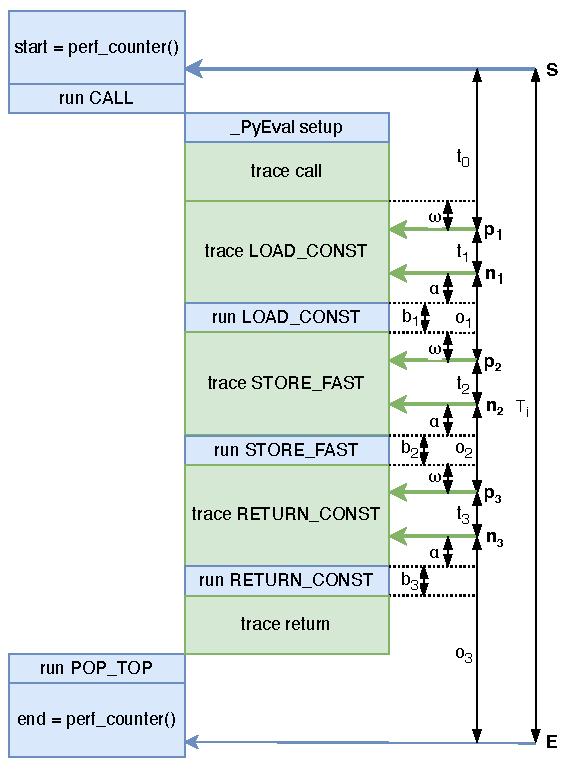
\includegraphics[width=\textwidth]{images/profiling_bytecode/traced_run.drawio.pdf}
       \caption{Fully traced function.}
       \label{figure:profiler-traced-run}
    \end{subfigure}
    \caption{.}
    \label{figure:profiler-run}
\end{figure}

%% From these, we can calculate the time taken by each opcode
% Hook
% Argument
% Link

\begin{equation}
    \label{eq:1}
    b_n = o_n - (\alpha + \omega)
\end{equation}

\begin{equation}
    \label{eq:2}
    \begin{split}
        T_i &= \sum_{n} t_n + \sum_{n} o_n \\
            &= T_u + n \alpha + n \omega
    \end{split}
\end{equation}

\begin{equation}
    \label{eq:3}
    b_n = o_n - \frac{T_i - T_u}{n}
\end{equation}

%% Timer granularity + other tricks
% Hook
Beyond the careful co-design of the tracing measurement logic with CPython's implementation, there are a number of confounding effects which must be mitigated to ensure accurate measurement.
% Argument
Firstly, for the profiling information to be useful, the resolution of the most accurate system clock must be sufficient to resolve differences bytecode execution time. On our experimental hardware (\autoref{ssec:experimental-setup}) this was true, having a $1$ns timer able to resolve differences in opcodes taking around $10$ns to execute. However, this is not the case for modern Apple Silicon devices. This is because their most accurate system timer, \texttt{mach\_absolute\_time} \cite{appleinc.Mach_absolute_time}, has a resolution of only $40$ns and is hence unable to resolve individual bytecode instruction durations of approximately $10$ns. This is a physical limitation on measuring such necessarily fast events, and as such can only be resolved by selecting appropriate hardware.
Secondly, the CPython language runtime periodically runs housekeeping tasks such as garbage collection, disrupting the flow of bytecode execution and hence adding random noise to our measurements. These can effects can be minimised using techniques from existing performance measurement work such as \texttt{timeit} \cite{pythonsoftwarefoundationTimeitMeasureExecution} or \texttt{pyperf} \cite{victorstinnerPsfPyperf2025}, for example by disabling garbage collection for the duration of profiling.
% Link
Finally, we repeat and aggregate our experimental measurements for statistical confidence, further minimising machine noise to ensure clean and reliable profiling results.


\section{Example usage}
\label{sec:profiling-bytecode-examples}

%% Simple
% Hook
Having implemented our profiler, we can demonstrate its capabilities on an example workload (Listing \ref{listing:profiler-example}).
% Argument
Each traced event is displayed on its own line, in combination showing the exact sequence of instructions performed by the interpreter when evaluating the function. Function invocations, such as calling \texttt{inner\_function} \circledbase{pairedOneLightBlue}{x}, are indented by their call stack depth for easy readability. In addition to this, bytecode instructions are formatted following the convention of the standard library, but are annotated with their duration in a comment on the right-hand side of the trace \circledbase{pairedTwoDarkBlue}{y}.
% Link


%% Listing function vs profiled bytecode
\begin{figure}[H]
    \centering
    \begin{subfigure}[b]{0.275\textwidth}
       \centering
        \begin{minted}[fontsize=\scriptsize,escapeinside=££]{python}
def inner_function(
    x: int | str | float
) -> None:
    assert x

def example_function():
    inner_function(1)
    pass
    _x = perf_counter()
        \end{minted}
        \footnotesize\vspace{8em}
        \caption{Python program.}
        \label{listing:profiler-example-python}
    \end{subfigure}
    \hfill
    \begin{subfigure}[b]{0.695\textwidth}
        \centering
        \begin{minted}[fontsize=\scriptsize,escapeinside=££,linenos=false]{text}
// ======= example:6 `example_function` ========
// >>> inner_function(1)
7           0   LOAD_GLOBAL          0   (inner_function)   // 15   ns
            2   LOAD_CONST           1   (1)                // 15   ns
            4   CALL_FUNCTION        1   ()                 // 31   ns

    // ======== example:1 `inner_function` ========= £\circledbase{pairedOneLightBlue}{\scriptsize{x}}£
    // >>> assert x
    4           0   LOAD_FAST            0   (x)            // 13   ns
                2   POP_JUMP_IF_TRUE     4   (to 8)         // 13   ns
            >>  8   LOAD_CONST           0   (None)         // 12   ns
                10  RETURN_VALUE             ()             // 31   ns
    // =============================================

            6   POP_TOP                  ()                 // 16   ns
// >>> pass
8           8   NOP                      ()                 // 15   ns £\circledbase{pairedTwoDarkBlue}{\scriptsize{y}}£
// >>> _x = perf_counter()
9           10  LOAD_GLOBAL          1   (perf_counter)     // 15   ns
            12  CALL_FUNCTION        0   ()                 // 17   ns
            14  STORE_FAST           0   (_x)               // 14   ns
            16  LOAD_CONST           0   (None)             // 13   ns
            18  RETURN_VALUE             ()                 // 28   ns
// =============================================
        \end{minted}
        \caption{Profiler output.}
        \label{listing:profiler-example-bytecode}
    \end{subfigure}
    \vspace{1em}
    \captionsetup{name=Listing}
    \caption{Output of the bytecode profiling tool for a simple Python program, showing the sequence of dispatched bytecode and their individual execution times.}
    \label{listing:profiler-example}
\end{figure}


%% Summary/why should I care?
% Hook
% Argument
% Link forward to where it is used in other places
% Link
